% Условная компиляция для самостоятельной работы
\ifdefined\mainfile
    % Если это часть основного файла, не добавляем начало и конец документа
\else
    \documentclass[12pt, a4paper]{report}
    \usepackage{/Users/vladbelousov/Desktop/Semestr_4-FP-NSU/Настройка/library}
    \usepackage[utf8]{inputenc} % Подключение поддержки UTF-8
    \begin{document}
\fi

%%-------------------------------%%

\section{Сведение задачи  об устойчивости  произвольного решения к задаче об устойчивости нулевого решения}

\[ \frac{d}{dt }  \vec{y} = \vec{f } (t, \vec{y} ) \tag{1}  \] 
\( \vec{y} ^{* } (t) \)  - решение, которое мы хотим исследовать на устойчивость. 

Предположим, что \( \vec{y } ^* (t) \) определенно от \( t_0 \) до \( +\infty  \).

Пусть \( \vec{y} (t) \)  - другое решение системы (1). Замена \( \vec{z }(t )= \vec{y } (t) - \vec{y }^{* } (t)   \) 

\[ \frac{d}{dt }  \vec{z } (t ) = \frac{d}{dt }  \vec{y} (t )- \frac{d}{dt }  \vec{y } ^*   (t ) = \vec{f } (t, \vec{y} (t))-\vec{f } (t, \vec{y } ^{* } (t)) =  \vec{f } (t, \vec{y}^* (t) +\vec{z } (t))-\vec{f } (t, \vec{y } ^{* } (t))\] 
\[ \frac{d}{dt }\vec{z } (t) =   \vec{f } (t, \vec{y}^* (t) +\vec{z } (t))-\vec{f } (t, \vec{y } ^{* } (t)) \tag{2} \] 

\( \vec{z } ^{* } (t) = 0\)  - решение системы (2). 

\begin{theorem}
    Решение \( \vec{y } ^{* } (t) \)  системы (1) устойчиво по Ляпунову/асимптотически устойчиво/неустойчиво \( \Leftrightarrow  \) нулевое решение \( \vec{z } ^{* } (t) = 0 \) системы (2) устойчиво по Ляпунову/асимптотически устойчиво/неустойчиво. 
\end{theorem}

\begin{proof} \(  \) 

По определению \( \vec{z } ^*   (t ) = 0 \) устойчиво по Ляпунову, если: 

1) \( \vec{z } ^* (t) = 0 \) определено от \( t_0 \) до \( +\infty  \) 

2) \( \exists  \Delta > 0 \text{ }  \forall  \vec{z } (t_0): \left\lVert  \vec{z } (t_0 )- \vec{z } ^* (t_0 ) \right\rVert < \Delta \Rightarrow \vec{z } (t) \) тоже определено от \( t_0 \) до \( \infty  \), где \( \vec{z} ^{* } (t_0 )= 0  \), а \( \vec{z } (t_0 )  = \vec{y } (t_0 )- \vec{y } ^* (t_0) \).

3) \( \forall  \varepsilon > 0 \text{ } \exists  \delta > 0  \text{ }  \forall  \vec{z } (t_0) : \left\lVert \vec{z } (t_0 ) - \vec{z } ^* (t_0 ) \right\rVert < \delta \Rightarrow \left\lVert \vec{z } (t ) - \vec{z } ^* (t) \right\rVert < \varepsilon \text{ }  \forall  t \ge  t_0 \), где   \( \vec{z} ^{* } (t_0 )= 0  \), а \( \vec{z } (t_0 )  = \vec{y } (t_0 )- \vec{y } ^* (t_0) \) и  где \( \vec{z} ^{* } (t )= 0  \), а \( \vec{z } (t)  = \vec{y } (t )- \vec{y } ^* (t) \)

\end{proof}

\[ \frac{d}{dt }  \vec{y } (t ) = A (t ) \vec{y } + \vec{ g } (t) = \vec{f } (t,\vec{y } )   \tag{3}  \] 
, где \( \displaystyle A(t ) = (a_{ij }(t) ) , \text{ }  \vec{g } (t ) = \begin{pmatrix}
g_1\\
\vdots\\
g_n
\end{pmatrix} , \text{ }  a_{ij }  (t ) , g_j(t )\in  C(\mathbb{R}) \) 

Так как система линейна, то любое решение определенно на \( \mathbb{R} \). 

\( \Rightarrow  \) пункты 1) и 2) в определении устойчивости выполнены автоматически. 

Замена \( \vec{z } (t) = \vec{y } (t )- \vec{y }^* (t)\), где  \( \vec{y } (t) \)   - другое решение (3). 

\[ \frac{d}{dt }  \vec{z }  = \vec{f } (t, \vec{y } ^* +\vec{z } ) - \vec{f } (t, \vec{y } ^*)  = A(t )\vec{z} \tag{4}\] 
, где \( \vec{z }^* (t )= 0 \)  - решение (4). 

\begin{theorem}
    Решение \( \vec{y } ^{* } (t) \) линейной неоднородной  системы (3) устойчиво по Ляпунову/асимптотически устойчиво/неустойчиво \( \Leftrightarrow  \) нулевое решение \( \vec{z } ^{* } (t) = 0 \) линейной неоднородной системы (4) устойчиво по Ляпунову/асимптотически устойчиво/неустойчиво. 
\end{theorem}

\textbf{Следствие 1.} На устойчивость решения линейной неоднородной системы (3) не влияет \( \vec{g } (t) \), а влияет  только \( A(t). \) 

\textbf{Следствие 2.} Все решения линейной системы (3) либо одновременно устойчивы, либо одновременно неустойчивы. 

\section{Устойчивость линейных системах}

\[ \frac{d}{dt }  \vec{y }  = A (t ) \vec{y } \tag{1}  \] 
, где \( \displaystyle  A (t ) = (a_{ij } (t)) , \text{ }  a_{ij }(t) \in  C(\mathbb{R})  \) 

\( \vec{y } ^* (t ) = 0 \) -  решение, которое мы исследуем на устойчивость. 

\begin{theorem}
    Нулевое решение  \( \vec{y } ^{* }  (t )  = 0 \) системы (1) устойчиво по Ляпунову \( \Leftrightarrow  \) все решения системы (1) ограничены вправо, то есть \( \forall   \) решения \( \vec{y } (t) \text{ }  \exists  M >0 \)  \( \left\lVert \vec{y} (t) \right\rVert \le M \text{  } \forall t \ge  t_0 \) 
\end{theorem}

\begin{proof} \(  \) 

    \( (\Rightarrow):\) 

    По определению: \( \forall  \varepsilon > 0 \text{ }  \exists  \delta > 0 \text{ }  \forall  \vec{y } _0 < \delta \Rightarrow \left\lVert \vec{y } (t) \right\rVert < \varepsilon \text{ }  \forall  t \ge  t_0 \) 


    Пусть \( \vec{y} (t ) \neq 0 \) - решение системы (1). Возьмем  \( \vec{v } (t ) =\displaystyle  \underbrace{\frac{\delta}{2 \left\lVert \vec{y } (t_0) \right\rVert }}_{\mathrm{const}   } \vec{y } ( t)  \) - тоже решение.

    \[ \left\lVert \vec{v} (t_0 ) \right\rVert  = \left\lVert \frac{ \delta }{2 \left\lVert \vec{y } (t_0 ) \right\rVert } \vec{y  } (t)  \right\rVert = \frac{ \delta }{2 \left\lVert \vec{y } (t_0) \right\rVert} \left\lVert \vec{y } (t_0) \right\rVert = \frac{\delta}{2 }  < \delta  \] 

    Из определения: \( \forall  \varepsilon > 0 \text{ } \exists  \delta > 0 \text{ }  \forall  \vec{v } (t ) : \left\lVert \vec{v }  (t_0) \right\rVert < \delta \Rightarrow \left\lVert \vec{v }  (t ) \right\rVert < \varepsilon \text{ }  \forall  t \ge  t_0 \) 

    \[ \left\lVert \frac{\delta }{2 \left\lVert  \vec{y } (t_0) \right\rVert } \vec{y } (t)  \right\rVert < \varepsilon \Rightarrow \left\lVert \vec{y } (t) \right\rVert < \varepsilon \frac{ 2 \left\lVert \vec{y } (t_0) \right\rVert}{\delta } = M  \] 

    \( (\Leftarrow): \) 

    Пусть \( \forall  \) решения \( \vec{y} (t ) \text{ } \exists  M > 0 : \left\lVert \vec{y } (t) \right\rVert \le  M \text{  } \forall  t \ge  t_0 \)  

    Все решения системы (1): \( \vec{y } (t ) = F(t ) \vec{c} = c_1 \vec{\varphi}_1 (t ) +... + c_n \vec{\varphi }_n(t)   \). 

    Возьмем \( F (t) \) - ФМР (фундаментальная матрица решений) такую, что \( F(t_0 ) = E\) 

    \[ \begin{aligned}
        \begin{cases}
            \displaystyle \frac{d}{dt }  \vec{ y } =   A(t )\vec{y } \\[5pt]
            \vec{y }  (t_0 )= \vec{y } _0
        \end{cases} 
        \Rightarrow \vec{y } (t ) = F(t ) \vec{c}= F(t ) \vec{y } _0 = y_{01} \vec{\varphi }_1 (t ) +...+ y_{0n }  \vec{\varphi }_n (t )   
    \end{aligned}\] 
    , где \( \displaystyle  \vec{y}_0 = \begin{pmatrix}
    y_{01}  \\
    \vdots\\
    y_{0n} 
    \end{pmatrix}, \text{ }  F(t ) = (\vec{\varphi }_1 (t ) |...|\vec{\varphi }_n(t)  )  \) 

    Так как \( \vec{\varphi }_1 (t ),..., \vec{\varphi }_n (t)   \) - решения, то \( \exists  M_1, \ldots, M_n : \left\lVert \vec{\varphi}_1  (t ) \right\rVert \le  M_1 ,..., \left\lVert  \vec{\varphi }_n (t) \right\rVert \le M_n \text{ }  \forall  r \ge  t_0 \) 

    Для решения задачи Коши: 

    \[ \left\lVert \vec{y } (t) \right\rVert  = \left\lVert y_{01} \vec{\varphi }_1 (t ) +...+ y_{0n } \vec{\varphi }_n(t)   \right\rVert \le \left\lvert y_{01} \right\rvert \left\lVert \vec{\varphi}_1 (t )  \right\rVert +...+ \left\lvert y_{0n }  \right\rvert \left\lVert  \vec{\varphi} _n (t) \right\rVert \le  \left\lvert y_{01} \right\rvert M_1+ ... + \left\lvert y_{0n}   \right\rvert M_n \le  \] 
    \[ \le  \underbrace{\max  \{M_1, \ldots, M_n\}}_{= \tilde{M}} (\left\lvert y_{01} \right\rvert + ...+ \left\lvert  y_{0n}  \right\rvert) = \tilde{M } \left\lVert \vec{y } _0 \right\rVert _1 \] 

    Возьмем норму \( \left\lVert \vec{y } _0 \right\rVert _1 = (\left\lvert y_{01} \right\rvert + ...+ \left\lvert y_{0n}  \right\rvert) \) 

    Если \( \left\lVert  \vec{y } _0  \right\rVert _ 1 < \delta \Rightarrow \left\lVert \vec{y } (t) \right\rVert  \le  \tilde{M } \left\lVert \vec{y} _0 \right\rVert _1  < \tilde{M }\delta \overset{(*)}{= }\varepsilon \), \( (*): \)  возьмем \( \delta =\displaystyle  \frac{\varepsilon}{\tilde{ M}}  \) 

    \( \Rightarrow  \vec{y } ^* (t) = 0\)  устойчиво по Ляпунову. 

\end{proof}

\begin{theorem}
    Нулевое решение \( \vec{y } ^{* } (t) = 0 \) системы (1) асимптотически устойчиво \( \Leftrightarrow  \) \( \forall  \) решения \( \vec{y } (t) \) выполняется \( \left\lVert \vec{y } (t) \right\rVert \xrightarrow{t \to  +\infty  } 0   \).
\end{theorem}

\begin{proof} \(  \) 

    \( (\Rightarrow): \) 

    Из определения асимптотической устойчивости: \( \exists  \rho> 0 \text{ }  \forall  \vec{y } _ 0 : \left\lVert \vec{y }  _0 \right\rVert < \rho \Leftrightarrow  \left\lVert \vec{y } (t) \right\rVert \xrightarrow{t \to  + \infty } 0   \) 

    Пусть \( \vec{y } (t)\neq 0  \)  - решение системы (1). Возьмем \( \vec{v } (t) =\displaystyle  \frac{ \rho }{2 \left\lVert \vec{y } (t_0) \right\rVert} \vec{y } (t)  \)  - тоже решение. 

    \[ \left\lVert \vec{v }  (t ) \right\rVert = \left\lVert \frac{\rho}{2 \left\lVert \vec{y } (t_0) \right\rVert} \vec{y } (t)   \right\rVert = \frac{\rho}{ 2 \left\lVert \vec{y } (t_0)  \right\rVert} \left\lVert \vec{y } (t_0) \right\rVert = \frac{\rho}{2 }  <\rho \] 

    \( \Rightarrow \) по определению асимптотической устойчивости: \( \displaystyle \lim_{t \to \infty } \left\lVert \vec{v} (t)  \right\rVert 0  \) 

    \[ \lim_{t  \to +\infty} \left\lVert \frac{\rho}{2 \left\lVert \vec{y } (t_0) \right\rVert } \vec{y} (t)  \right\rVert = 0 \Rightarrow \lim_{t \to +\infty}  \left\lVert \vec{y } (t) \right\rVert = 0 \] 

    \( (\Leftarrow): \) 

    Пусть \( \forall   \) решения \( \vec{y } (t) \)  выполняется \( \displaystyle \left\lVert \vec{y } (t) \right\rVert \xrightarrow{ t \to  + \infty } 0    \) 

    Хотим доказать:
    
    1) \( \vec{y } ^* (t)  \) устойчиво по Ляпунову. По Теореме 1. достаточно доказать, что все решения ограничены вправо. 

    По определению предела: \( \displaystyle  \left\lVert \vec{y } (t ) \right\rVert \xrightarrow{ t \to  +\infty } 0   \) 

    \[ \forall  \sigma > 0 \text{ }  \exists  T \text{ }  \forall  t \ge  T : \left\lVert \vec{y } (t) \right\rVert < \sigma \]  

    \( \vec{y } (t) \) - непрерывна, \( [t_0, T] \) - компакт \( \Rightarrow \left\lVert \vec{y } (t) \right\rVert \le  c \text{ }  \forall  t \in  [t_0 , T] \) 

    \( \Rightarrow \left\lVert  \vec{y } (t) \right\rVert \le  \max  \{\sigma, c \} , t \ge  t_0 \Rightarrow  \)  по Теореме 1. \( \vec{y } ^* (t ) = 0  \) устойчиво по Ляпунову. \\

    2) Надо проверить: \( \exists  \rho > 0 \text{ } \forall  \vec{y } _0 : \left\lVert \vec{y } _0  \right\rVert < \rho \Rightarrow \displaystyle \lim_{t \to +\infty} \left\lVert \vec{y } (t) \right\rVert = 0  \) 

    \begin{center}
        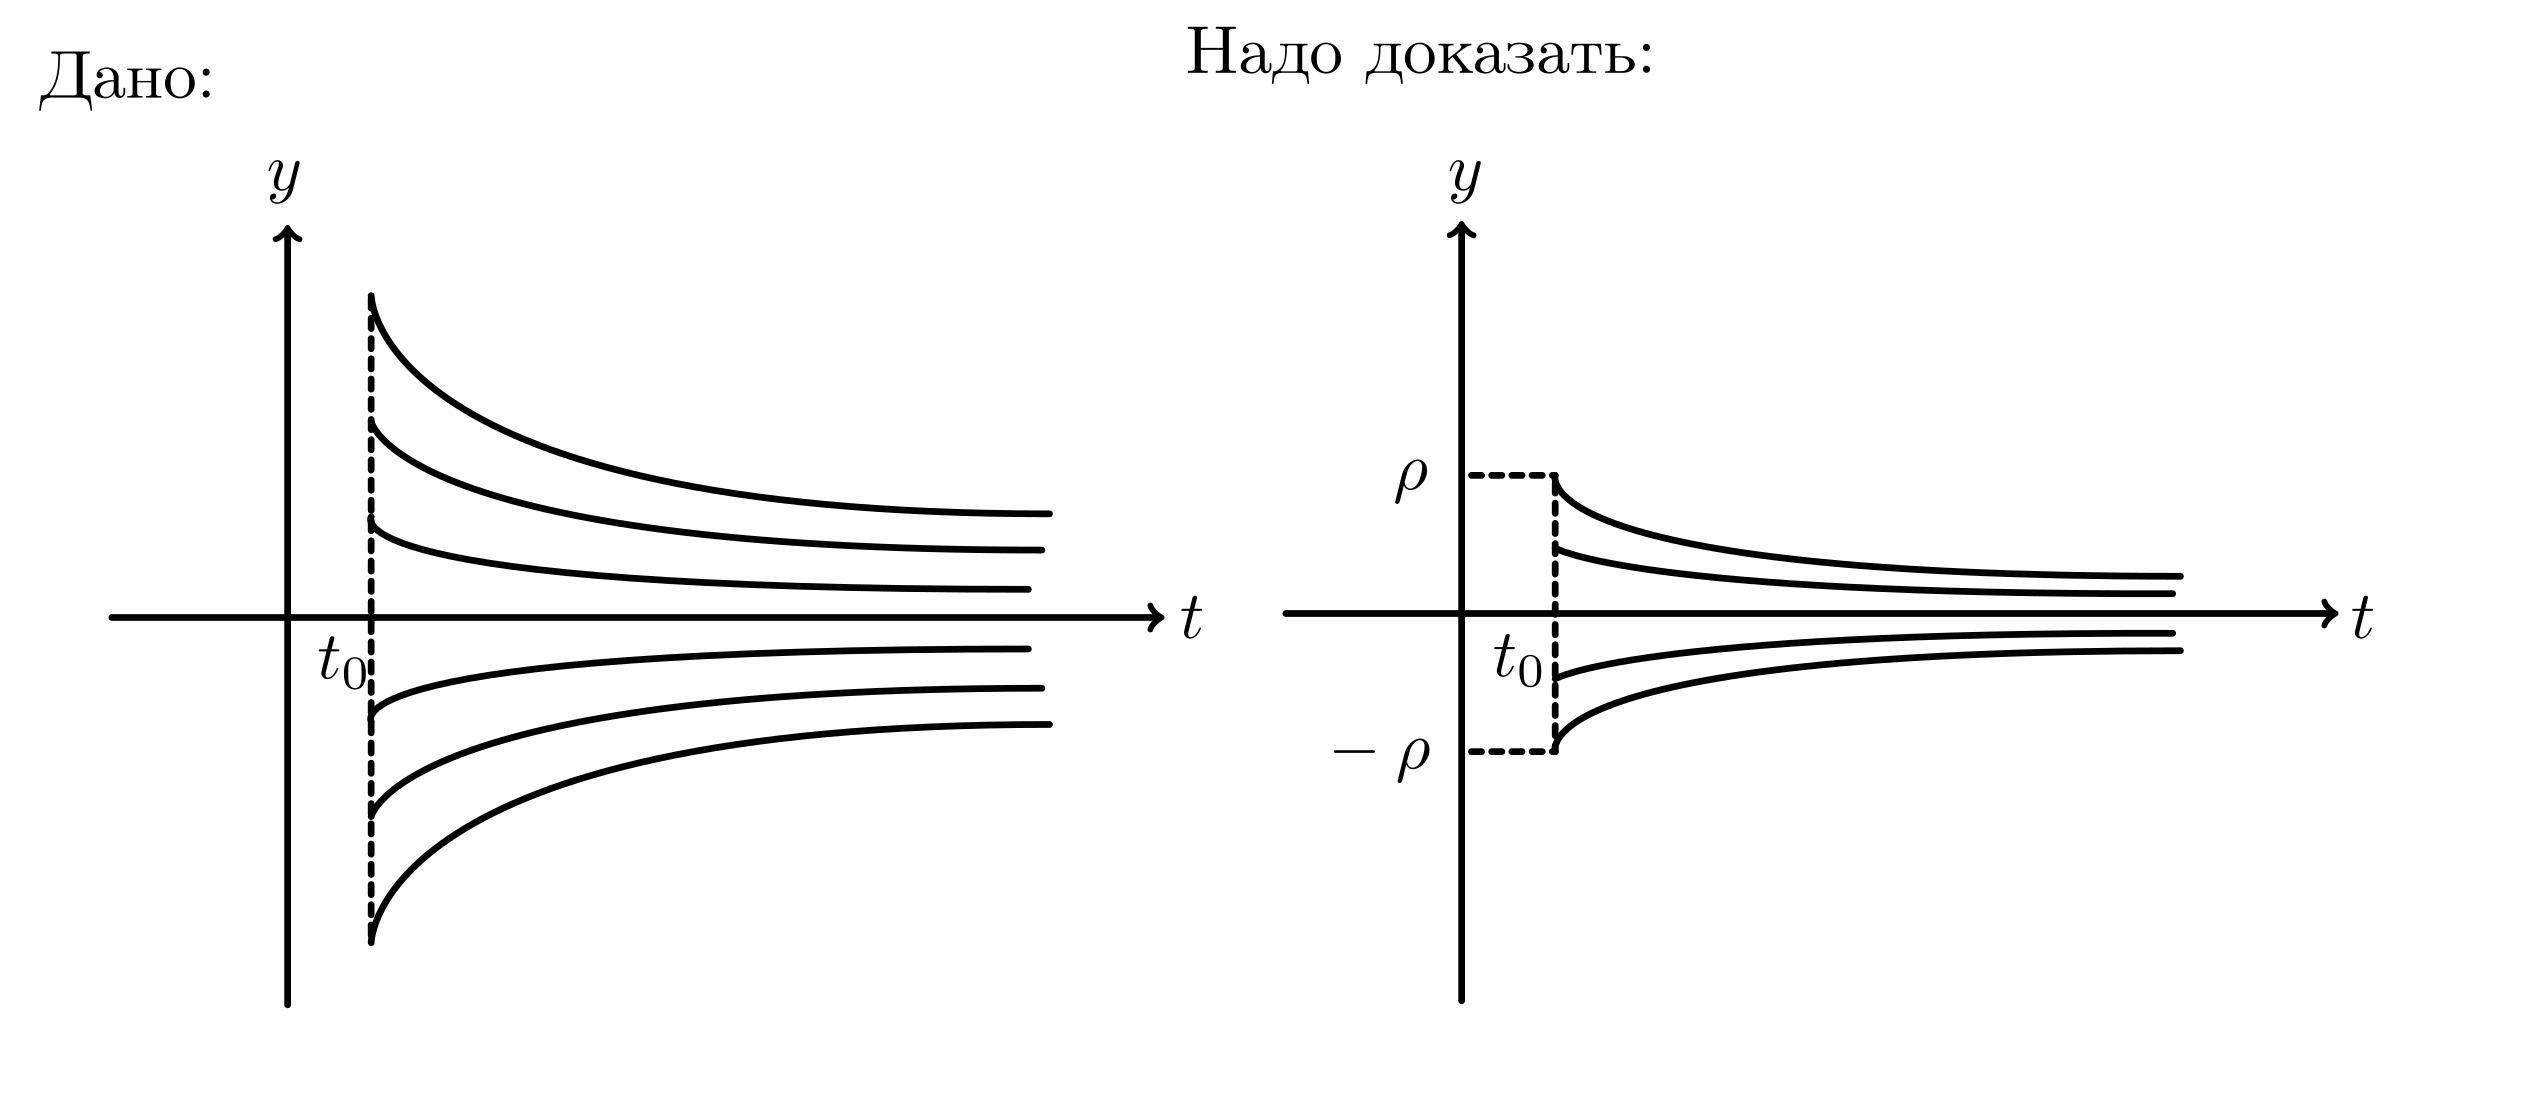
\includegraphics[width=0.84\textwidth]{/Users/vladbelousov/Desktop/Semestr_4-FP-NSU/ДфУ/Лекции_по_дням/image/44.png}
    \end{center}


    Возьмем \( \rho = 1 \), тогда 2) пункт выполняется. 

    \[ \vec{ y } ^{* } (t )  = 0  \text{ асимптотически устойчиво.} \] 

\end{proof}

\[ \frac{d}{dt }  \vec{y } = A y \tag{2} \] 
, где \( \displaystyle  A (t ) = (a_{ij } ) , \text{ }  a_{ij } \in  C(\mathbb{R})  \)

Все решения \( \vec{y } (t) = e^{ t A }  \vec{ c }  = T e^{ t Y }  \vec{b} \).



%%-------------------------------%%

% Закрытие документа, если файл компилируется отдельно
\ifdefined\mainfile
    % Если это основной файл, не нужно заканчивать документ
\else
    \end{document}
\fi